\documentclass[conference]{IEEEtran}
\IEEEoverridecommandlockouts
\usepackage{cite}
\usepackage{amsmath,amssymb,amsfonts}
\usepackage{mathtools}
\usepackage{algorithmic}
\usepackage{graphicx}
\usepackage{booktabs}
\usepackage{textcomp}
\usepackage{xcolor}
\usepackage{url}
\usepackage{dblfloatfix}
\usepackage{float}
\usepackage{placeins}
\allowdisplaybreaks[1]
\setcounter{topnumber}{3}
\setcounter{dbltopnumber}{2}
\setcounter{totalnumber}{4}
\renewcommand{\topfraction}{0.95}
\renewcommand{\bottomfraction}{0.90}
\renewcommand{\dbltopfraction}{0.95}
\renewcommand{\textfraction}{0.05}
\renewcommand{\floatpagefraction}{0.70}
\renewcommand{\dblfloatpagefraction}{0.70}
\setlength{\textfloatsep}{10pt plus 2pt minus 2pt}
\setlength{\dbltextfloatsep}{10pt plus 2pt minus 2pt}
\setlength{\floatsep}{9pt plus 2pt minus 2pt}
\makeatletter
\setlength{\@fptop}{0pt}
\setlength{\@fpsep}{10pt}
\setlength{\@fpbot}{0pt plus 1fil}
\setlength{\@dblfptop}{0pt}
\setlength{\@dblfpsep}{10pt}
\setlength{\@dblfpbot}{0pt plus 1fil}
\makeatother
\DeclareMathOperator*{\argmin}{arg\,min}
\DeclareMathOperator*{\argmax}{arg\,max}
\def\BibTeX{{\rm B\kern-.05em{\sc i\kern-.025em b}\kern-.08em
T\kern-.1667em\lower.7ex\hbox{E}\kern-.125emX}}

\title{RouteCast: Calibrated Cross-Token Expert Forecasting with Selective Cache-Aware Prefetching for Heterogeneous MoE Models}

\author{\IEEEauthorblockN{Jihua Dong}
\IEEEauthorblockA{\textit{School of Microelectronics} \\
\textit{University of Electronic Science and Technology of China}\\
Chengdu, China \\
2023190903038@std.uestc.edu.cn}}

\begin{document}
\maketitle
\begin{abstract}
Sparse mixture-of-experts (MoE) inference may place expert-weight transfers on
the critical path when selected experts are not resident in accelerator memory.
Prefetching can hide these transfers, but inaccurate predictions increase data
movement and pollute limited expert caches. We present RouteCast, a route-only
framework that couples expert forecasting with selective prefetching. A
context-conditioned gate integrates six complementary evidence branches:
layer popularity, one-hop transitions, two-hop transitions, request-prefill
popularity, GRU history, and multiscale frequency and recency. RouteCast
calibrates marginal expert-inclusion probabilities, adapts the candidate
budget using validation-selected cumulative score mass, and admits only
candidates whose temperature-scaled ranking weight exceeds that of
the cache entry they would replace. The framework requires neither hidden
states nor modifications to
the native router.

We evaluate RouteCast using request-disjoint traces comprising 1,000 requests
from each of three heterogeneous MoE architectures: Qwen3, DeepSeek-R1, and
Llama 4 Maverick. Under their native expert budgets, RouteCast achieves Recall
values of 0.5558, 0.3172, and 0.3602, respectively. These results exceed
matched temporal convolutional network (TCN) predictors by 2.81, 4.55, and
5.79 percentage points, corresponding to relative improvements of 5.3\%,
16.7\%, and 19.1\%. RouteCast also consistently outperforms paper-derived and
request-aware heatmap baselines across the three routing regimes. Confidence
intervals from 10,000 paired request-level bootstrap resamples exclude zero
for all three RouteCast--TCN comparisons. Component ablations identify GRU
history as a consistent contributor, while the utility of individual
statistical priors varies across routing regimes. One shared predictor is
within 0.0007 macro-average Recall of three independently trained predictors;
Group-DRO changes macro Recall by less than 0.0001 and is not credited with a
Recall gain. Budget sweeps reveal
explicit trade-offs between
expert coverage and transfer volume, while idealized trace-driven cache-event replay shows
that selective admission reduces unnecessary transfers relative to unfiltered
adaptive prefetching. Together, these results establish RouteCast as an
interface between marginally calibrated route prediction and budget-aware expert
prefetching. The present trace-based evaluation does not establish
end-to-end latency improvements in a deployed MoE system.
\end{abstract}


\begin{IEEEkeywords}
sparse mixture-of-experts, route-only prediction, expert prefetching,
marginal confidence calibration, adaptive candidate budget, cache-aware scheduling
\end{IEEEkeywords}

\section{Introduction}
Sparse mixture-of-experts (MoE) language models increase parameter capacity
while activating only a small subset of experts for each token
\cite{shazeer2017,gshard,switch}. This
conditional computation reduces arithmetic cost, but the complete expert pool
may still exceed accelerator memory. In an offloaded deployment, an expert
that is not resident must be transferred from host memory or another device
after it is selected by the native router. Because this transfer occurs
between routing and expert execution, reactive loading can expose
data-movement latency on the inference critical path.

Speculative expert prefetching attempts to transfer likely experts before they
are requested. Previous studies have explored router co-design, proactive
expert movement, and sparsity-aware caching
\cite{pregated,moeinfinity,promoe}. Public route traces further indicate that
expert selections exhibit exploitable spatial and temporal structure
\cite{patterns}. Prediction recall alone, however, is insufficient. Enlarging
the candidate set can trivially cover more true experts, but it also increases
false transfers, cache pollution, and replacement pressure. A practical
prefetching method must therefore address three coupled questions: which
experts are likely to be selected, how reliable are the predicted scores, and
which predictions should be converted into physical transfers under a finite
cache budget?

We study these questions under a route-only constraint. RouteCast observes
discrete expert identifiers from earlier token positions together with
structural metadata, but it does not access hidden activations or
native-router logits. This constraint makes the predictor applicable when
route traces are available but modifying the serving model is undesirable. It
also creates a difficult forecasting problem across heterogeneous routing
regimes. Qwen3 and DeepSeek-R1 select eight experts from model-specific expert
pools, whereas Llama 4 Maverick selects a single expert. Consequently, a fixed
heuristic or a predictor tuned to one architecture may not transfer reliably
to another.

\begin{figure*}[!t]
\centering
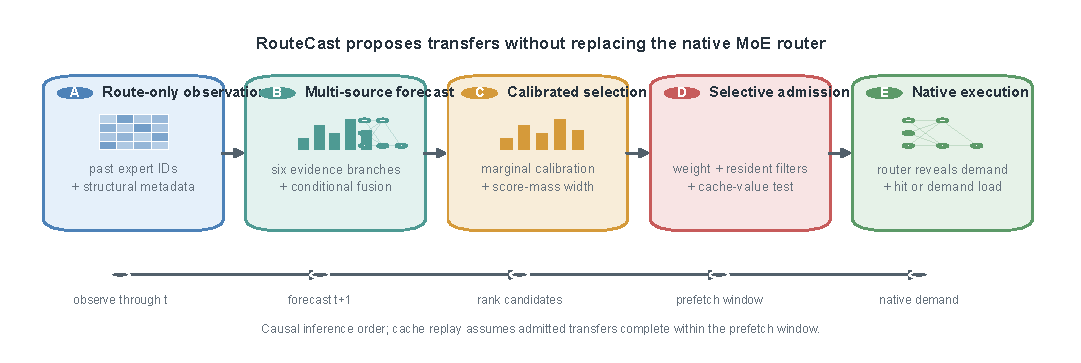
\includegraphics[width=0.97\textwidth]{figures_final/Fig1_RouteCastOverview}
\caption{RouteCast pipeline from route observation to selective expert
prefetching. Previously observed expert identifiers and structural metadata
feed a multi-source forecaster. Calibrated selection converts its scores into
an adaptive candidate set, and cache-aware admission decides which candidates
should trigger speculative movement. The lower timeline states when each
decision is made; the frozen native router remains authoritative over the
experts that execute.}
\label{fig:framework}
\end{figure*}

Figure~\ref{fig:framework} provides the system-level view. The detailed
forecaster is introduced with Fig.~\ref{fig:forecaster}, whereas
Fig.~\ref{fig:selection-admission} separates calibration, adaptive candidate
selection, and cache admission. This hierarchy prevents implementation details
from obscuring the central distinction between forecasting quality, candidate
coverage, and cache behavior.

The study makes three contributions:

\begin{itemize}
    \item We establish a request-disjoint protocol for next-token expert
    forecasting across three heterogeneous public MoE trace families. The
    protocol preserves model-specific native expert budgets and reports
    ranking quality under matched train, validation, and test partitions.

    \item We introduce a route-only predictor that combines four statistical
    priors with GRU history and multiscale frequency--recency evidence through a
    context-conditioned probability-mixture gate. The predictor requires
    neither hidden states nor modifications to the native router. A single
    shared checkpoint retains nearly the same macro-average Recall as three
    independently trained predictors across the evaluated architectures.

    \item We connect marginal expert calibration to adaptive candidate
    selection, low-weight rejection, and cache-aware admission. Budget sweeps,
    component ablations, request-level bootstrap analysis, and trace-driven
    idealized cache-event replay jointly characterize prediction gains, transfer trade-offs,
    and model--capacity failure boundaries.
\end{itemize}

The resulting evidence is algorithmic and trace-driven. It establishes the
quality of route forecasting and selective prefetch decisions, but it does not
demonstrate end-to-end latency, throughput, or energy improvements in a
deployed MoE serving system.


\section{Related Work}

\textbf{MoE inference and expert movement.}
Memory-constrained MoE inference commonly places inactive experts in host
memory or secondary storage and transfers them to the accelerator on demand.
Large-scale MoE systems have consequently developed specialized parallelism,
communication, and execution support for sparse expert computation
\cite{deepspeedmoe,tutel}; CPU--GPU orchestration provides another route to
serving models whose expert weights exceed accelerator memory
\cite{fiddler}.
Pre-gated MoE co-designs expert selection and execution to overlap expert
movement with useful computation \cite{pregated}. MoE-Infinity exploits
activation sparsity through a sparsity-aware expert cache on
memory-constrained machines \cite{moeinfinity}, whereas ProMoE investigates
proactive expert caching for MoE serving \cite{promoe}. These studies
demonstrate that expert movement can be hidden or avoided through prediction,
caching, and execution overlap. Their end-to-end gains, however, necessarily
depend on deployment-specific factors such as cache capacity, transfer
bandwidth, scheduling policy, and available computation overlap. RouteCast
focuses on the complementary problem of producing marginally calibrated expert forecasts
before those predictions are consumed by a particular runtime.

\textbf{Expert-route forecasting.}
\emph{Patterns behind Chaos} identifies spatial and temporal regularities in
expert-selection traces and provides the public trace data used in this study
\cite{patterns}. Related spatio-temporal predictors exploit dependencies
across tokens or layers to estimate future expert selections \cite{stmoe}.
These observations establish that historical routes contain predictive
information, but the usefulness of each dependency can vary across models,
requests, layers, and routing regimes. RouteCast therefore treats route
statistics as conditionally informative evidence rather than applying a fixed
fusion rule. Its gate combines layer popularity, one-hop and two-hop
transitions, request-prefill popularity, GRU history, and multiscale
frequency--recency evidence without using hidden activations or native-router
logits.

\textbf{From prediction to prefetch action.}
Recent speculative prefetching methods increasingly recognize that a correct
ranking is useful only when candidate transfers can be issued early and
without excessive cache disruption \cite{specmd,specprefetch}. This distinction
is important because increasing the prefetch width can improve expert coverage
while simultaneously increasing false transfers and cache pollution.
RouteCast makes this distinction explicit by evaluating expert ranking,
candidate selection, and cache action separately. Fixed-budget metrics measure
the forecaster, while idealized trace-driven replay measures cache hits, transfer volume,
and wasted prefetches. Increased expert coverage is therefore not interpreted
as an equivalent end-to-end speedup.

\section{RouteCast Design}
\subsection{Problem Formulation and Design Principles}

For request \(r\) from model family \(g\), token position \(t\), and routed
layer \(\ell\), let \(E_g\) denote the number of candidate experts and \(K_g\)
the native routing width. The routing decision is represented by
\(\mathbf{y}_{r,t,\ell}^{(g)}\in\{0,1\}^{E_g}\), where
\(\|\mathbf{y}_{r,t,\ell}^{(g)}\|_0=K_g\). Its non-zero entries define the
executed expert set \(\mathcal{Y}_{r,t,\ell}^{(g)}\).

RouteCast predicts the expert set at the same routed layer for the next token:
\begin{align}
\mathbf{s}_{r,t+1,\ell}^{(g)}
&=
f_{\theta}\!\left(
\mathcal{R}_{r,\leq t},
\mathbf{c}_{r,t,\ell}
\right), \\
\widehat{\mathcal{Y}}_{r,t+1,\ell}^{(g,K_g)}
&=
\operatorname{TopK}\!\left(
\mathbf{s}_{r,t+1,\ell}^{(g)},K_g
\right).
\label{eq:task}
\end{align}
Here, $\mathcal{R}_{r,\leq t}$ is the sequence of expert identifiers observed
up to token $t$, and $\mathbf{c}_{r,t,\ell}$ is a five-dimensional structural
context vector. It contains the normalized layer position, expert-pool size,
native routing sparsity, request-prefill entropy, and token position. The
function \(f_{\theta}\) denotes the RouteCast predictor with trainable
parameters \(\theta\), while
\(\mathbf{s}_{r,t+1,\ell}^{(g)}\in\mathbb{R}^{E_g}\) contains one score for
each candidate expert. The operator \(\operatorname{TopK}(\cdot,K_g)\)
returns the \(K_g\) highest-scoring experts.

The prediction problem is heterogeneous across the evaluated traces, as shown
in Table~\ref{tab:route-regimes}. Qwen3 and DeepSeek-R1 share a native routing
width of eight but differ by a factor of two in expert-pool size. Llama 4 Maverick
Maverick instead adopts Top-1 routing and contains substantially fewer routed
layers. The resulting 22.38 million token-layer instances therefore span
different output dimensions, positive-label densities, and temporal routing
structures.

\begin{table}[!t]
\centering
\caption{Routing and training configurations. \(E_g\) is the expert-pool size,
\(K_g\) the native routing width, \(L_g\) the number of routed layers, and
\(\mathcal{K}_g\) the multi-budget training set.}
\label{tab:route-regimes}
\scriptsize
\setlength{\tabcolsep}{2.3pt}
\begin{tabular}{@{}lrrrrl@{}}
\toprule
Model & \(E_g\) & \(K_g\) & \(L_g\) & Train inst. & \(\mathcal{K}_g\) \\
\midrule
Qwen3             & 128 & 8 & 94 & 8.34M & \(\{8,12,16\}\) \\
DeepSeek-R1       & 256 & 8 & 58 & 5.20M & \(\{8,12,16\}\) \\
Llama 4 Maverick  & 128 & 1 & 24 & 2.17M & \(\{1,2,4,8\}\) \\
\bottomrule
\end{tabular}
\end{table}

All learned transformations share parameters along the expert axis, and the
gate consumes fixed-dimensional summaries rather than a flattened expert
vector. The same predictor can therefore process different \(E_g\) values
without a model-specific output head.

RouteCast is route-only and causal. It uses neither hidden activations nor
native-router logits, and it observes no information from token $t+1$ when
forming its prediction. The native router remains authoritative: RouteCast may
propose an expert transfer, but it cannot change which experts are executed. A
false positive therefore causes an unnecessary speculative transfer, whereas a
false negative leaves the corresponding demand transfer unhidden.

RouteCast further separates marginal calibration, score normalization, and
prefetch action. Temperature-scaled sigmoid outputs \(\mathbf{q}\) represent
marginal expert-inclusion probabilities and are evaluated by BCE, Brier score,
and ECE. A separate softmax produces unit-sum ranking weights \(\mathbf{w}\),
which control candidate width but are not interpreted as categorical
probabilities for multi-label Top-\(K\) routing. The admission policy receives
\(\mathbf{w}\), cache state \(\mathcal{C}_{r,t}^{(g)}\), score-mass threshold
\(m_g^*\), and admission threshold \(\tau_g^*\). It may prefetch fewer than
\(K_g\) experts or abstain completely.

This separation allows forecasting quality, candidate coverage, and cache
behavior to be evaluated independently. Forecasting is first evaluated under
the native budget \(K_g\), preventing a method from appearing more accurate
merely because it predicts more experts. Adaptive selection is then evaluated
through Recall, Precision, and mean candidate width, while idealized cache replay
measures hit rate, issued transfers, and wasted prefetches. Consequently, an
increase in candidate coverage is not automatically interpreted as an
equivalent improvement in system performance.
\subsection{Multi-Source Route Forecasting}

For request \(r\) from model family \(g\), RouteCast predicts the route at
token \(t+1\) and layer \(\ell\) from observations through token \(t\). It
constructs six per-expert branches: layer popularity, one-hop transition,
two-hop transition, request-prefill popularity, GRU history, and multiscale
frequency--recency evidence. The first four are empirical priors; the final
two learn request-local departures over a history of \(H=16\) tokens. For
readability, request and model superscripts are omitted from branch variables
when their identity is unambiguous.

\subsubsection{Statistical route evidence}

Let \(E_g\) denote the number of experts in model group \(g\), and let
\(\mathcal{Y}_{r,t,\ell}^{(g)}\) be the set observed at token \(t\) and
layer \(\ell\). Layer popularity is the normalized training count
\(q_{\ell,e}^{\mathrm{pop}}=N_{\ell}^{\mathrm{pop}}(e)/
\sum_jN_{\ell}^{\mathrm{pop}}(j)\), where
\(N_{\ell}^{\mathrm{pop}}(e)\) counts selections of expert \(e\) at layer
\(\ell\).

The one-hop branch normalizes the sum of empirical transition rows
\(\mathbf{A}_{\ell,u}^{(1)}\) for
\(u\in\mathcal{Y}_{r,t,\ell}^{(g)}\). The two-hop branch applies the analogous
matrix \(\mathbf{A}_{\ell,u}^{(2)}\) to experts observed at token \(t-1\).

Request-prefill popularity normalizes the corresponding within-request count
\(N_{r,\ell}^{\mathrm{pre}}(e)\) over experts at layer \(\ell\).

When a transition or prefill count is empty, the corresponding branch falls
back to layer popularity. Transition statistics are computed from training requests;
the request-prefill prior uses only the observed prefill of the current
request.

\subsubsection{Learned temporal evidence}

Let \(\mathbf{x}_{t,\ell,e}=[x_{t-H+1,\ell,e},\ldots,
x_{t,\ell,e}]^{\top}\in\{0,1\}^{H}\) denote the activation history of expert
\(e\), where
\(x_{\tau,\ell,e}=1\) if expert \(e\) was selected at token \(\tau\) and
layer \(\ell\), and zero otherwise. RouteCast uses \(H=16\). Histories shorter
than \(H\) are left-padded with zeros.

The recurrent score is
\(z_{t,\ell,e}^{\mathrm{gru}}=\mathbf{w}_{\mathrm{gru}}^{\top}
\operatorname{GRU}(\mathbf{x}_{t,\ell,e})+b_{\mathrm{gru}}\), using a shared
GRU \cite{cho2014} with hidden dimension 24. Sharing the GRU across experts
allows the branch to learn recurring activation patterns without assigning an
independent temporal model to every expert.

The multiscale branch complements the GRU with mean activation over windows
\(\mathcal{W}=\{1,2,4,8,H\}\) and a normalized recency feature. Let
\(\mu_{t,\ell,e}^{(w)}\) denote the mean activation within the most recent
\(w\) tokens and \(\rho_{t,\ell,e}\) the recency of the latest activation.
The resulting feature vector is
\(\mathbf{u}_{t,\ell,e}=[\mu^{(1)},\mu^{(2)},\mu^{(4)},\mu^{(8)},
\mu^{(H)},\rho]_{t,\ell,e}\). A two-layer MLP with a 24-dimensional hidden
layer and GELU activation produces
\(z_{t,\ell,e}^{\mathrm{multi}}=f_{\mathrm{multi}}
(\mathbf{u}_{t,\ell,e})\).

The GRU can learn nonlinear sequential dependencies, whereas the multiscale
branch exposes short- and long-range frequency changes directly. Their
combination avoids requiring one temporal encoder to represent both types of
behavior.

\subsubsection{Distribution-level conditional fusion}

The four statistical probabilities are converted to scores using
\(\operatorname{logit}(\operatorname{clip}(q,\epsilon,1-\epsilon))\), while
the GRU and multiscale networks directly produce learned scores. Let
\(\mathbf{z}_{t,\ell}^{(b)}\in\mathbb{R}^{E_g}\) denote the score vector for
branch \(b\in\{1,\ldots,6\}\). Each branch is independently normalized over
its expert dimension:

\begin{equation}
p_{t,\ell,e}^{(b)}
=
\frac{
\exp\!\left(z_{t,\ell,e}^{(b)}\right)
}{
\displaystyle
\sum_{j=1}^{E_g}
\exp\!\left(z_{t,\ell,j}^{(b)}\right)
}.
\label{eq:branch-normalization}
\end{equation}

This produces six comparable expert distributions, irrespective of their
original score scales.

The gate does not process all \(E_g\) probabilities directly. Each branch is
summarized by its maximum probability, Top-1/Top-2 margin, and normalized
entropy \(\mathcal{H}(\mathbf{p})=-\sum_e p_e\log p_e/\log E_g\). These 18
descriptor values are concatenated with five structural variables: normalized
layer position, expert-pool size, native sparsity, request-prefill entropy, and
normalized token position. A \(23\!\rightarrow\!64\!\rightarrow\!6\) MLP with
GELU activation and softmax output produces non-negative branch weights
\(\boldsymbol{\omega}_{r,t,\ell}^{(g)}\) that sum to one.

The gate first forms a probability mixture and then converts it into a log
score with an expert-specific residual correction:
\begin{align}
p_{t,\ell,e}^{\mathrm{mix}}
=
\sum_{b=1}^{B_{\mathrm{br}}}
\omega_{r,t,\ell}^{(b)}
p_{t,\ell,e}^{(b)},\\
s_{t,\ell,e}
=
\log
p_{t,\ell,e}^{\mathrm{mix}}
+
\alpha \Delta_{t,\ell,e},
\qquad
\alpha=0.1.
\label{eq:fusion}
\end{align}

The residual \(\Delta_{t,\ell,e}\) is produced by a lightweight MLP with dimensions
\(10\rightarrow32\rightarrow1\) and GELU activation. Its input contains the
four statistical features, their transformed branch scores, the GRU score,
and the multiscale score for expert \(e\). The output layer is initialized to
zero, so optimization begins from pure probability-mixture fusion and learns
a correction only when supported by the training data.

All branch transformations act independently along the expert axis and share
parameters across experts. The descriptor and context dimensions are fixed,
so the same network supports different \(E_g\) values without a
model-specific output head. Distribution-level fusion prevents branches with numerically larger raw
scores from dominating the mixture. The context-conditioned gate can assign
different evidence weights across layers, requests, token positions, and model
families. It can therefore emphasize a branch when its distribution is sharp
and structurally appropriate, or suppress it when the same signal becomes
diffuse or unreliable under another routing regime.

\begin{figure*}[!t]
\centering
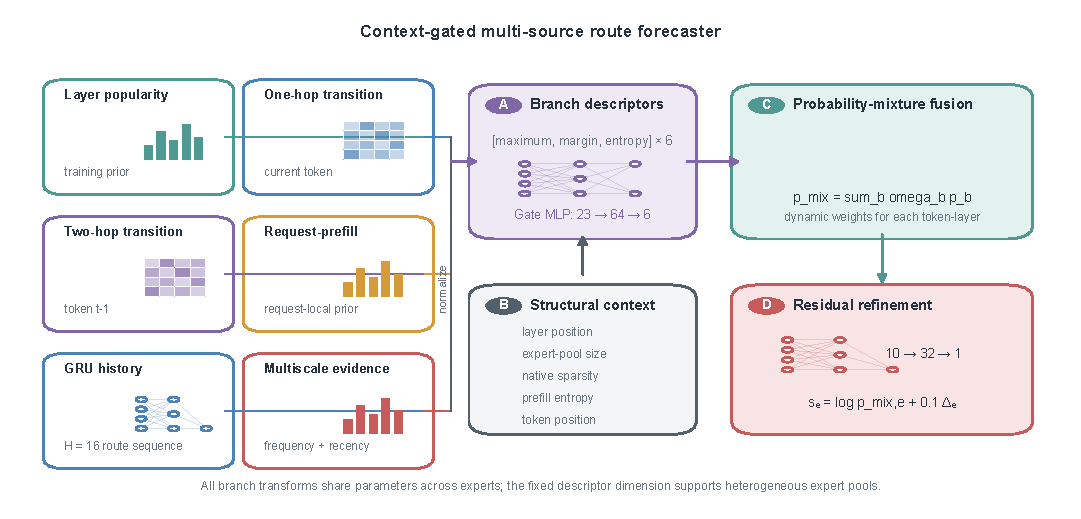
\includegraphics[width=0.96\textwidth]{figures_final/Fig2_MultiSourceForecaster}
\caption{Context-gated multi-source route forecaster. Six statistical and
learned temporal branches are normalized independently. Their concentration,
margin, and entropy descriptors are combined with structural context by a
small gating network, producing token--layer-specific mixture weights. A
lightweight residual network refines the mixture score without introducing a
model-specific expert-output head.}
\label{fig:forecaster}
\end{figure*}

Figure~\ref{fig:forecaster} maps the equations in this subsection to the
implemented computation graph. The branch cards show the six evidence sources;
the middle blocks distinguish distribution descriptors from structural
context; and the right-hand blocks show conditional mixture fusion followed by
the bounded residual correction.

\subsection{Cross-Model Learning}
\label{sec:cross-model-learning}

RouteCast uses a shared parameter set across all three model families rather
than training an independent predictor for each architecture. Joint training
exposes the predictor to heterogeneous routing regimes, but it also introduces
substantial imbalance. As summarized in Table~\ref{tab:route-regimes}, the
request-disjoint training split contains
15.71 million token--layer instances, including 8.34 million from Qwen3,
5.20 million from DeepSeek-R1, and 2.17 million from Llama 4 Maverick.
The models also differ in expert-pool size, native routing width, and evaluated
prefetch budgets. Naively pooling these instances would therefore bias the
shared predictor toward the largest trace family and routing regime.

For a training instance from model group \(g\), let
\(\mathbf{s}_{g}\in\mathbb{R}^{E_g}\) denote the predicted expert-score vector
and \(\mathbf{y}_{g}\in\{0,1\}^{E_g}\) the corresponding multi-hot target.
The number of positive entries in \(\mathbf{y}_g\) is the native routing width
\(K_g\). RouteCast minimizes the weighted objective

\begin{equation}
\begin{split}
\mathcal{L}_{g} ={}&
0.20\,\mathcal{L}_{\mathrm{BCE}}
+0.25\,\mathcal{L}_{\mathrm{list}} \\
&+0.35\,\mathcal{L}_{\mathrm{rank}}
+0.20\,\mathcal{L}_{\mathrm{budget}}\,.
\end{split}
\label{eq:total-loss}
\end{equation}

The four terms address complementary prediction errors.
The class-balanced binary cross-entropy
\(\mathcal{L}_{\mathrm{BCE}}\) provides expert-wise supervision. Because only
\(K_g\) of the \(E_g\) experts are positive, positive labels are assigned
weight \((E_g-K_g)/K_g\). The listwise term
\(\mathcal{L}_{\mathrm{list}}\) instead supervises the complete ranking. It
uses \(\mathbf{y}_g/K_g\) as the target distribution and minimizes its
negative log-likelihood under
\(\operatorname{softmax}(\mathbf{s}_g)\). Division by \(\log E_g\) makes the
loss scale more comparable across expert pools of different sizes.

The remaining terms focus on errors near the prefetch cutoff. The ranking term
compares every true expert with the 24 highest-scoring false experts using a
softplus pairwise penalty. The budget term applies the same penalty whenever a
true expert falls below a model-specific Top-\(k\) boundary in
\(\mathcal{K}_g\) (Table~\ref{tab:route-regimes}). These terms concentrate
optimization on mistakes that change either the native candidate set or the
coverage--transfer curve.

RouteCast combines static sample-count balancing with Group-DRO
\cite{sagawa2020}. A group containing \(n_g\) of the \(n\) training instances
receives static factor \(a_g=n/(3n_g)\). Adaptive weights start uniformly and
are updated with exponentiated mean group loss using step size
\(\eta_{\mathrm{dro}}=0.8\). The effective contribution of group \(g\) is
\(3a_gd_g\mathcal{L}_g\). The primary-evaluation ablation below shows that this
adaptive reweighting did not materially change Recall, so it is treated as a
training control rather than a source of a Recall gain.

Training uses AdamW \cite{loshchilov2019} with a learning rate of \(6\times10^{-4}\), weight decay
of \(10^{-4}\), and a batch size of 256. Mixed precision is used for the
forward pass, while loss reductions are performed in FP32 and Group-DRO
weights are normalized in float64. The implementation checks inputs, scores,
losses, and gradients for non-finite values and clips the gradient norm to
1.0. The final checkpoint is selected by the macro-average native-budget
validation Recall, defined as the unweighted mean of
\(\operatorname{Recall@}K_g\) over the three model groups. Each routing regime
therefore contributes equally to model selection, irrespective of trace size.

We isolate the effects of parameter sharing and adaptive group reweighting in
two matched ablations. The first retains one shared predictor and static
sample-count balancing but fixes the three group weights uniformly. The second
trains an independent predictor for each model family. Both use the same
architecture, loss, request splits, seed, batch size, and number of epochs as
the primary model. These controls distinguish gains from the RouteCast
architecture from gains attributable specifically to cross-model sharing or
Group-DRO.
\subsection{Marginal Calibration and Score-Mass Selection}

The fused scores determine an expert ranking, but their numerical scale is not
directly comparable across model families. RouteCast first calibrates marginal
expert-inclusion probabilities separately for each model family. It then uses
a distinct unit-sum normalization to control candidate width. Keeping these
two quantities separate is essential for multi-label routing.

Let \(g\in\{1,\ldots,G\}\) index a model family. We suppress the request
index in this subsection when it is unambiguous. Let
\(s_{t,\ell,e}^{(g)}\) be the fused score assigned to expert \(e\) for token
position \(t\) and routed layer \(\ell\). A positive temperature \(T_g^*\) is
selected by minimizing binary cross-entropy on the validation split, following
the single-parameter temperature-scaling procedure of Guo et al.
\cite{guo2017}:

\begin{align}
T_g^*
&=\argmin_{T>0}\operatorname{BCE}_{\mathrm{val},g}
\!\left(\mathbf{s}^{(g)}/T,\mathbf{y}^{(g)}\right), \\
q_{t,\ell,e}^{(g)}
&=\sigma\!\left(s_{t,\ell,e}^{(g)}/T_g^*\right), \\
w_{t,\ell,e}^{(g)}
&=\frac{\exp(s_{t,\ell,e}^{(g)}/T_g^*)}
{\sum_{j=1}^{E_g}\exp(s_{t,\ell,j}^{(g)}/T_g^*)}.
\label{eq:calibrated-quantities}
\end{align}

where \(\mathbf{s}^{(g)}\) and \(\mathbf{y}^{(g)}\) collect the validation
scores and multi-hot expert targets for model \(g\), respectively. The
temperature is optimized while all RouteCast parameters remain frozen.
Because division by a positive scalar does not change score ordering,
temperature scaling preserves every fixed-budget Top-\(K\) prediction while
adjusting score concentration. Equation~\eqref{eq:calibrated-quantities}
then defines two distinct quantities. Marginal probabilities \(q\) determine
the reported BCE, Brier score, and ECE, whereas unit-sum weights \(w\) control
candidate selection. Here, \(E_g\) is the number of routed experts and
\(\sum_{e=1}^{E_g}w_{t,\ell,e}^{(g)}=1\). For Top-\(K\) routers with
\(K>1\), \(w_{t,\ell,e}^{(g)}\) is not a categorical probability because
multiple experts can be correct simultaneously. It is a normalized ranking
weight used only to convert score concentration into a candidate budget.

Let
\(w_{t,\ell,(1)}^{(g)}
\geq\cdots\geq
w_{t,\ell,(E_g)}^{(g)}\)
denote the sorted ranking weights. Given a cumulative score-mass threshold
\(m\in(0,1]\), RouteCast selects the smallest prefix whose normalized weight
reaches \(m\):

\begin{equation}
K_{t,\ell}^{(g)}(m)
=
\min
\left\{
k\in\{1,\ldots,K_{\max,g}\}:
\sum_{i=1}^{k}
w_{t,\ell,(i)}^{(g)}
\geq m
\right\}.
\label{eq:adaptive-width}
\end{equation}

Here, \(K_{\max,g}\) is the largest permitted candidate width. If the threshold
is not reached within this limit, RouteCast uses \(K_{\max,g}\). The candidate
set contains the first \(K_{t,\ell}^{(g)}(m)\) experts in the ranking. A
concentrated score vector therefore produces a smaller set than a diffuse one.

The operating score mass is selected on validation data rather than assigned
a probabilistic coverage interpretation or fixed globally. Let
\(\overline{K}_g(m)\) denote mean candidate width over validation instances.
Let \(R_{\mathrm{val},g}(m)\) be the corresponding validation Recall and
\(R_{\mathrm{val},g}(K_g)\) the Recall obtained with the native fixed width
\(K_g\). RouteCast selects

\begin{equation}
\begin{aligned}
m_g^*
={}&
\argmin_{m\in\mathcal{M}}
\overline{K}_{g}(m) \\
\text{subject to}\quad
&
R_{\mathrm{val},g}(m)
\geq
\rho\,
R_{\mathrm{val},g}(K_g),
\qquad
\rho=0.98,
\end{aligned}
\label{eq:mass-selection}
\end{equation}

where \(\mathcal{M}\) is the evaluated mass grid and \(\rho\) is the required
Recall-retention ratio. If the constraint is infeasible, RouteCast selects the
candidate mass with the highest validation Recall, breaking ties in favor of a
smaller mean width. This procedure yields a
model-specific operating point \(m_g^*\), rather than imposing one threshold
on heterogeneous routers with different expert-pool sizes, native widths, and
score concentrations.


\subsection{Selective Cache Admission}

Adaptive score mass determines which experts are plausible, but it does not imply
that every candidate should trigger a transfer. RouteCast therefore applies
low-weight rejection and cache-aware admission before issuing speculative
movement. These decisions affect only prefetch behavior; the native router
remains authoritative over expert execution.

For model \(g\), an admission-weight threshold \(\tau_g\) is selected using the
validation split. Given threshold \(\tau\), let \(U_g^{+}(\tau)\) and
\(U_g^{-}(\tau)\) denote the mean numbers of correct and incorrect issued
candidates per prediction instance. RouteCast chooses

\begin{equation}
\tau_g^*
=
\argmax_{\tau\in\mathcal{T}}
\left[
U_g^{+}(\tau)
-
\lambda_{\mathrm{w}}U_g^{-}(\tau)
\right],
\qquad
\lambda_{\mathrm{w}}=1,
\label{eq:abstention-threshold}
\end{equation}

where \(\mathcal{T}\) is the evaluated threshold set and
\(\lambda_{\mathrm{w}}\) controls the penalty assigned to an incorrect
speculative candidate. Ties are resolved in favor of issuing fewer
candidates. The threshold set includes a value greater than one, so complete
abstention remains a valid zero-utility fallback when all speculative
predictions have negative validation utility.

After score-mass selection, RouteCast retains candidates in
\(\mathcal{P}_{t,\ell}^{(g)}(m_g^*)\) only when their ranking weight satisfies
\(w_{t,\ell,e}^{(g)}\geq\tau_g^*\).

Candidates already resident in the cache are removed because they require no
movement. A cache entry is represented by a layer--expert pair
\(c=(\ell,e)\). Let \(\mathcal{C}_t\) be the set of resident entries before
processing token \(t\), and let \(C_{\max,g}\) denote cache capacity. Each resident
entry maintains value \(v_t(c)\). A current ranking weight refreshes this
value; otherwise RouteCast applies exponential decay
\(v_t(c)=0.90v_{t-1}(c)\).

The decay prevents an entry supported only by stale predictions from retaining
high cache priority indefinitely. If
\(|\mathcal{C}_t|<C_{\max,g}\), a non-resident candidate is admitted without eviction.
When the cache is full, RouteCast identifies the least-valued resident entry
\(c_t^*=\argmin_{c\in\mathcal{C}_t}v_t(c)\) and applies the admission rule

\begin{equation}
\operatorname{Admit}_t(a)
=
\begin{cases}
1,
&
w_{t,\ell,a}^{(g)}
>
v_t(c_t^*)+\delta, \\[2pt]
0,
&
\text{otherwise},
\end{cases}
\qquad
\delta=0,
\label{eq:cache-admission}
\end{equation}

for each non-resident candidate \(a\). If
\(\operatorname{Admit}_t(a)=1\), candidate \(a\) replaces \(c_t^*\);
otherwise, RouteCast abstains from moving it. The margin \(\delta\) controls
how much more valuable a candidate must be than the entry it would evict. We
use \(\delta=0\), which still requires every replacement to provide a strictly
larger temperature-scaled ranking weight.

The complete decision sequence is ranking, adaptive score-mass selection,
low-weight rejection, resident filtering, and cache admission, as summarized in
Fig.~\ref{fig:selection-admission}.

A wrong forecast can cause an unnecessary speculative transfer or an
unfavorable cache replacement, but it cannot change the router-selected
experts or the numerical output of the MoE model. Prediction quality and cache
utility are consequently evaluated as separate outcomes.

\begin{figure*}[!t]
\centering
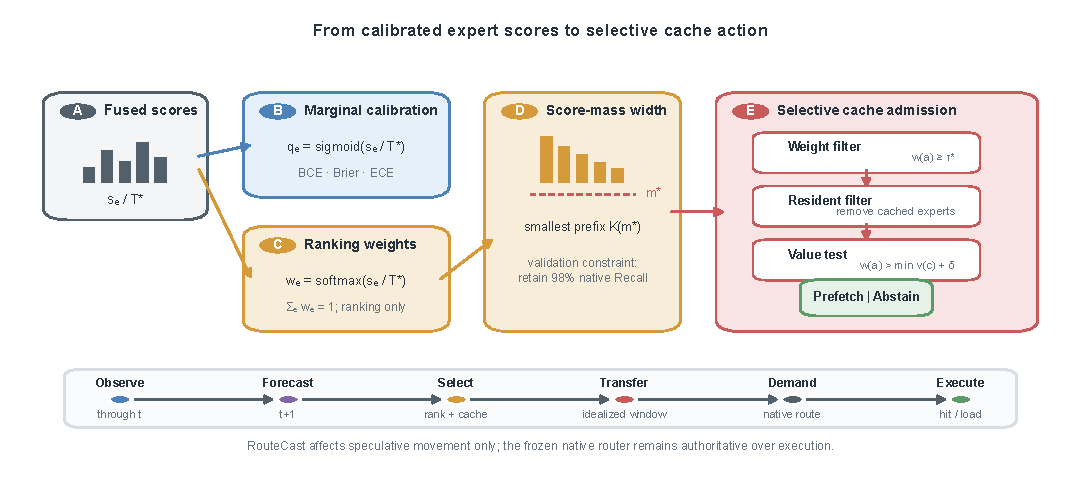
\includegraphics[width=0.96\textwidth]{figures_final/Fig3_SelectionAdmission}
\caption{Calibrated candidate selection and selective cache admission.
Temperature-scaled logits define sigmoid marginal inclusion probabilities for
calibration assessment and, separately, unit-sum softmax ranking weights for
score-mass selection. The selected prefix is filtered by admission weight,
cache residency, and relative cache value before RouteCast issues a prefetch or
abstains. The lower strip shows the causal inference timeline used by the
idealized trace-driven replay.}
\label{fig:selection-admission}
\end{figure*}

Figure~\ref{fig:selection-admission} makes the two uses of temperature-scaled
scores explicit. Marginal probabilities support BCE, Brier score, and ECE;
ranking weights determine candidate width and admission priority. Neither
quantity changes the native router's final expert selection.

\section{Experimental Design}
\subsection{Trace Data and Request-Disjoint Splits}

We evaluate RouteCast on the public expert-selection traces released with
\emph{Patterns behind Chaos} \cite{patterns}. The traces cover
Qwen3-235B-A22B-FP8, DeepSeek-R1-AWQ, and
Llama-4-Maverick-17B-128E-Instruct. Their routing configurations are reported
in Table~\ref{tab:route-regimes}. We retain the first 1,000 complete request
files available for each model family.

Requests are assigned deterministically to training, validation, and test
sets. We normalize each relative request path to use forward slashes, compute
its SHA-1 digest, interpret the first four bytes as an unsigned big-endian
integer, and divide by \(2^{32}\). Hash values below 0.70 enter training,
values in \([0.70,0.85)\) enter validation, and the remainder enter testing.
All token--layer records belonging to one request remain in the same split.
Consequently, neither adjacent tokens nor layers from a test request can
appear during training or model selection. The split is independent of the
optimization seed.

\begin{table*}[!t]
\centering
\caption{Request-disjoint composition of the primary 1,000-request-per-model
evaluation. Example counts refer to eligible next-token, same-layer prediction
instances after constructing histories of length \(H=16\).}
\label{tab:data-splits}
\scriptsize
\setlength{\tabcolsep}{4.2pt}
\begin{tabular}{@{}lrrrrrr@{}}
\toprule
& \multicolumn{3}{c}{Requests} & \multicolumn{3}{c}{Token--layer examples} \\
\cmidrule(lr){2-4}\cmidrule(lr){5-7}
Model & Train & Validation & Test & Train & Validation & Test \\
\midrule
Qwen3 & 698 & 145 & 157 & 8,343,910 & 1,733,736 & 1,885,170 \\
DeepSeek-R1 & 708 & 139 & 153 & 5,199,528 & 1,022,736 & 1,123,638 \\
Llama 4 Maverick & 708 & 145 & 147 & 2,171,400 & 445,440 & 450,672 \\
\midrule
Total & 2,114 & 429 & 457 & 15,714,838 & 3,201,912 & 3,459,480 \\
\bottomrule
\end{tabular}
\end{table*}

The resulting packed representation contains 22,376,230 prediction examples
from 3,000 requests. A complete numeric audit covers every cached tensor and
finds no non-finite value. Statistical and request-prefill counts are formed
only from the permitted training or observed request context. Test labels are
used only for final evaluation.

\subsection{Prediction Task and Matched Comparators}

Each example predicts the expert set at token \(t+1\) and routed layer
\(\ell\) from routes observed through token \(t\). The primary comparison uses
the native expert budget, \(K_g=8\) for Qwen3 and DeepSeek-R1 and \(K_g=1\)
for Llama 4 Maverick. Budget sweeps additionally evaluate
\(\{8,12,16\}\) for Qwen3 and DeepSeek-R1 and \(\{1,2,4,8\}\) for Llama 4 Maverick
Maverick. Predictions never alter the native routing labels.

We compare RouteCast with four route-only baselines. \emph{Paper Heatmap}
implements the cross-token transition estimator derived from the trace study
\cite{patterns}. \emph{Request-aware Heatmap} augments this estimator with
statistics accumulated from the observed portion of the current request.
\emph{GRU-only} receives the same 16-token binary route history as RouteCast
but excludes its statistical, multiscale, and gated-fusion branches.
\emph{TCN-only} replaces the recurrent branch with four causal dilated
convolution blocks using dilation factors 1, 2, 4, and 8, following the generic
temporal convolutional architecture of Bai et al. \cite{bai2018}. It receives no
RouteCast prior or gating feature.

All learned methods use the same request split, prediction targets, candidate
budgets, three-epoch schedule, and checkpoint rule. Their checkpoints maximize
validation macro-averaged native-budget Recall across the three model
families. They also share the loss and Group-DRO procedure in
Section~\ref{sec:cross-model-learning}. Heatmap statistics are estimated from training requests only
and require no gradient-based optimization. This protocol changes model
architecture while holding the available route information and evaluation
conditions fixed.

\subsection{Metrics and Statistical Analysis}

Let \(\mathcal{P}_i^{(K)}\) and \(\mathcal{Y}_i\) denote the predicted Top-\(K\)
set and the true expert set for token--layer example \(i\). Forecasting quality
is measured as
\begin{align}
\operatorname{Recall@K}
&=\frac{1}{N}\sum_{i=1}^{N}
\frac{|\mathcal{P}_i^{(K)}\cap\mathcal{Y}_i|}{|\mathcal{Y}_i|},\\
\operatorname{Precision@K}
&=\frac{1}{N}\sum_{i=1}^{N}
\frac{|\mathcal{P}_i^{(K)}\cap\mathcal{Y}_i|}{K}.
\label{eq:evaluation-metrics}
\end{align}
We also report the mean number of true experts recovered per example. Mean
reciprocal rank (MRR) uses the rank of the first relevant expert. NDCG@\(K\)
discounts later relevant experts logarithmically and normalizes by the ideal
ranking for the same target set \cite{jarvelin2002}. Under native-budget evaluation,
\(|\mathcal{Y}_i|=K_g=K\), so Recall and Precision are numerically equal.
They diverge when the candidate budget differs from the native routing width.

Marginal expert calibration is evaluated with binary cross-entropy (BCE),
Brier score, and expected calibration error (ECE). Adaptive selection reports mean candidate
width, candidate Recall, issued-prefetch coverage, issued-prefetch Precision,
and abstention rate. Idealized cache replay reports demand hit rate, on-demand loads,
prefetch loads, useful and wasted prefetches, prefetch Precision, and total
expert transfers.

Uncertainty is quantified with a paired request-level bootstrap
\cite{efron1993}. For each
model comparison, 10,000 resamples draw complete test requests with replacement
and recompute the pooled metric difference between RouteCast and its matched
baseline. Pairing preserves the same sampled requests for both methods, while
request-level sampling retains dependence among tokens and layers within a
request. We report percentile 95\% confidence intervals using bootstrap seed
2026. No token--layer record is treated as an independent bootstrap unit.

\subsection{Development Analyses and Idealized Cache Replay}

The 1,000-request-per-model split supplies the primary forecasting comparison
and request-level bootstrap analysis. A separate 100-request-per-model
development-scale evaluation is used for module ablation, candidate-budget sweeps,
temperature-scaling diagnostics, three-seed screening, and idealized cache replay. This
separation keeps the principal forecasting table at the largest evaluated
trace scale while allowing diagnostic experiments to remain computationally
tractable. Results from the development-scale evaluation are identified explicitly and
are not pooled with the primary test set.

The idealized trace-driven cache-event replay compares four policies:
demand-only least recently used
(LRU), fixed native-budget prefetching, unfiltered adaptive-mass prefetching,
and the complete policy with adaptive score mass, low-weight rejection, resident
filtering, and value-based admission. The cache is reset at each request and
is warm-started with experts observed before the first eligible prediction.
For model \(g\), capacity is
\(C_{\max,g}=cL_gK_g\), where
\(c\in\{1,2,4\}\). Resident values decay by \(\beta=0.90\), and replacements
require a strictly larger candidate value with \(\delta=0\).

At each replay step, RouteCast first constructs candidates from past routes,
then applies the selected admission policy, and finally reveals the native
route as demand. A prefetched expert is useful only if it is demanded before
eviction. Total transfers equal on-demand loads plus speculative prefetch
loads, and prefetch Precision is the fraction of prefetch loads used before
eviction. Every admitted speculative load is assumed to complete before its
corresponding demand. Replay therefore models cache-event ordering, residency,
and transfer counts, but not transfer deadlines, expert sizes, bandwidth,
kernel execution, communication overlap, or contention. It provides an
idealized upper bound on residency benefit and supports only cache-event and
movement-count claims, not prefetch feasibility, latency, or throughput claims.

\subsection{Implementation and Reproducibility}

RouteCast and the learned baselines are implemented in PyTorch. Training uses
AdamW \cite{loshchilov2019} with batch size 256, learning rate \(6\times10^{-4}\), weight decay
\(10^{-4}\), gradient clipping at 1.0, and three epochs. The primary tables
use seed 2026; development-scale stability checks additionally use seeds 2024
and 2025. Per-model temperatures are fitted on validation data with L-BFGS
while the predictor remains frozen. All candidate-mass and confidence
thresholds are also selected exclusively on validation data.

Experiments were run under Windows with Python 3.12.13, PyTorch
2.13.0+cu126, CUDA 12.6, and an NVIDIA GeForce RTX 4060 Laptop GPU. Cached-data
manifests and principal training scripts are recorded by SHA-256 digest. The
implementation uses finite-value checks, FP32 loss reduction, float64
normalization of Group-DRO weights, and gradient clipping to prevent numerical
failures from being silently incorporated into reported checkpoints.

\section{Results}
\subsection{RouteCast Improves Cross-Model Forecasting}

The primary 1,000-request-per-model evaluation is summarized in
Table~\ref{tab:main} and Fig.~\ref{fig:main}. RouteCast achieved native-budget
Recall of 0.5558 on Qwen3, 0.3172 on DeepSeek-R1, and 0.3602 on Llama 4
Maverick. It also obtained the highest MRR and NDCG among the evaluated
methods for every model.

TCN-only was the stronger of the two matched temporal baselines by
native-budget Recall. RouteCast exceeded TCN-only by 0.0281 on Qwen3, 0.0455
on DeepSeek-R1, and 0.0579 on Llama 4 Maverick. The corresponding paired
request-level 95\% confidence intervals were \([0.0265,0.0299]\),
\([0.0403,0.0510]\), and \([0.0546,0.0610]\), respectively. Each interval
excluded zero. RouteCast also exceeded GRU-only on all three models. These
comparisons isolate gains beyond recurrent or convolutional encoding of route
history alone.

\begin{figure*}[!t]
\centering
\begin{minipage}[c]{0.64\textwidth}
\centering
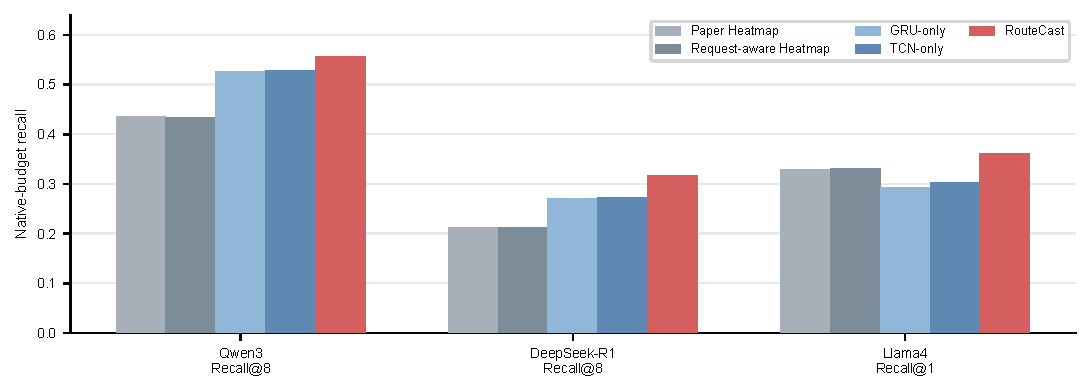
\includegraphics[width=\linewidth]{figures_final/Fig2a_MainComparison}
\end{minipage}\hfill
\begin{minipage}[c]{0.33\textwidth}
\centering
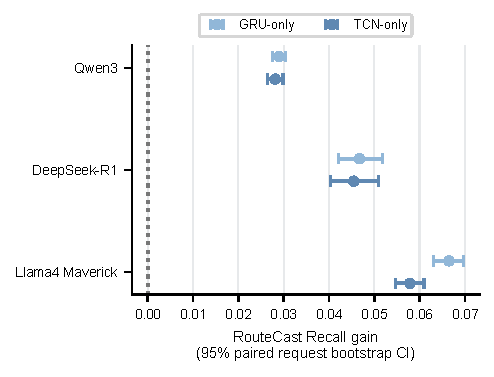
\includegraphics[width=\linewidth]{figures_final/Fig2b_RequestBootstrap}
\end{minipage}
\caption{Cross-model forecasting on the primary 1,000-request-per-model
evaluation. Left: native-budget Recall under matched request-disjoint splits.
Right: paired RouteCast Recall differences relative to GRU-only and TCN-only;
error bars denote 95\% request-level bootstrap confidence intervals.}
\label{fig:main}
\end{figure*}

Matched training with seeds 2024, 2025, and 2026 provided a development-scale
robustness check. RouteCast exceeded TCN-only for every model under every seed
(Fig.~\ref{fig:tcn-seeds}). The request-level bootstrap on the primary evaluation
remains the principal uncertainty analysis.

\begin{table}[!t]
\centering
\caption{Native-budget forecasting on the primary 1,000-request-per-model
evaluation. Precision equals Recall because predicted and true sets have the
same cardinality.}
\label{tab:main}
\scriptsize
\setlength{\tabcolsep}{2.4pt}
\begin{tabular}{llccc}
\toprule
Model & Method & Recall & MRR & NDCG \\
\midrule
Qwen3 & Heatmap & .4352 & .7969 & .4859 \\
& Request-aware & .4330 & .7956 & .4834 \\
& GRU-only & .5268 & .8893 & .5903 \\
& TCN-only & .5277 & .8902 & .5936 \\
& \textbf{RouteCast} & \textbf{.5558} & \textbf{.9013} & \textbf{.6208} \\
\midrule
DeepSeek-R1 & Heatmap & .2131 & .5087 & .2413 \\
& Request-aware & .2121 & .5076 & .2402 \\
& GRU-only & .2705 & .6715 & .3243 \\
& TCN-only & .2717 & .6707 & .3265 \\
& \textbf{RouteCast} & \textbf{.3172} & \textbf{.7131} & \textbf{.3743} \\
\midrule
Llama 4 M. & Heatmap & .3298 & .4593 & .3298 \\
& Request-aware & .3311 & .4653 & .3311 \\
& GRU-only & .2938 & .4470 & .2938 \\
& TCN-only & .3024 & .4451 & .3024 \\
& \textbf{RouteCast} & \textbf{.3602} & \textbf{.4988} & \textbf{.3602} \\
\bottomrule
\end{tabular}
\end{table}

\subsection{Shared Training Retains Similar Macro Recall}

Table~\ref{tab:cross-model-ablation} separates the effects of shared training
and Group-DRO. Replacing adaptive Group-DRO weights with uniform group weights
changed macro Recall by only 0.000093. Three independent predictors exceeded
the shared model by 0.000646 macro Recall, with mixed model-level directions.
The shared checkpoint therefore preserved similar aggregate Recall, but
neither parameter sharing nor Group-DRO produced a uniform gain. Because this
ablation used one seed, the differences do not establish statistical
equivalence.

\begin{table}[!t]
\centering
\caption{Cross-model training ablation on the primary 1,000-request-per-model
split with seed 2026. Values are native-budget Recall. Shared denotes static
sample balancing with uniform group weights; per-model trains one independent
predictor for each architecture.}
\label{tab:cross-model-ablation}
\scriptsize
\setlength{\tabcolsep}{2.7pt}
\begin{tabular}{lccc}
\toprule
Model & Shared+DRO & Shared & Per-model \\
\midrule
Qwen3 & .555837 & .555895 & .558416 \\
DeepSeek-R1 & .317227 & .316581 & .312466 \\
Llama 4 M. & .360242 & .361107 & .364363 \\
\midrule
Macro average & .411102 & .411195 & .411748 \\
\bottomrule
\end{tabular}
\end{table}

\subsection{Budget Expansion Reveals Model-Specific Cost}

Fixed-width sweeps on the development-scale evaluation increased coverage at the cost of
lower prefetch Precision (Fig.~\ref{fig:budget}). For Qwen3, increasing
\(K\) from 8 to 16 raised Recall from 0.5835 to 0.7886, while the false-prefetch
fraction increased from 0.4165 to 0.6057. DeepSeek-R1 reached only 0.3618
Recall at \(K=16\), where 0.8191 of predictions were false. For Llama 4 Maverick,
increasing \(K\) from 1 to 8 raised Recall from 0.2848 to 0.6540,
but the false-prefetch fraction reached 0.9183. Candidate width therefore
controlled a model-dependent coverage--movement trade-off rather than
prediction quality alone.

\begin{figure*}[!t]
\centering
\begin{minipage}[c]{0.67\textwidth}
\centering
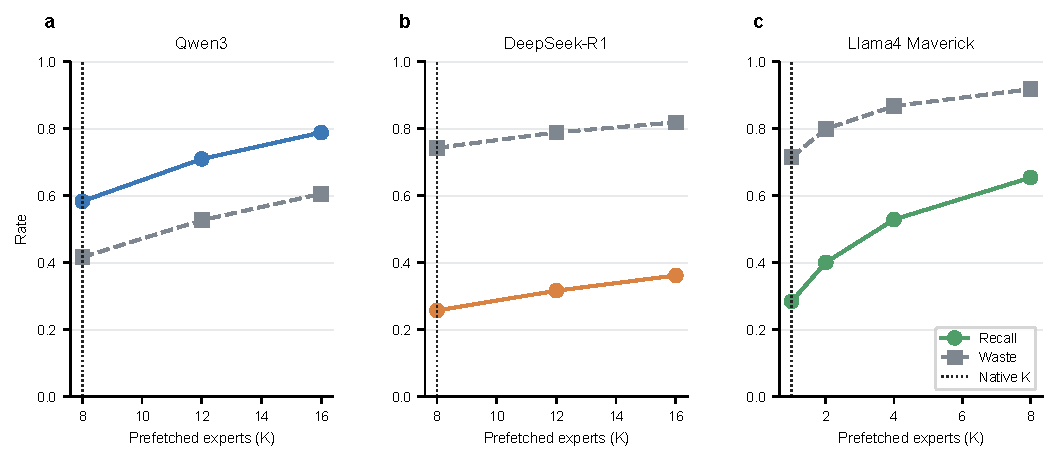
\includegraphics[width=\linewidth]{figures_final/Fig3_BudgetTradeoff}
\end{minipage}\hfill
\begin{minipage}[c]{0.30\textwidth}
\centering
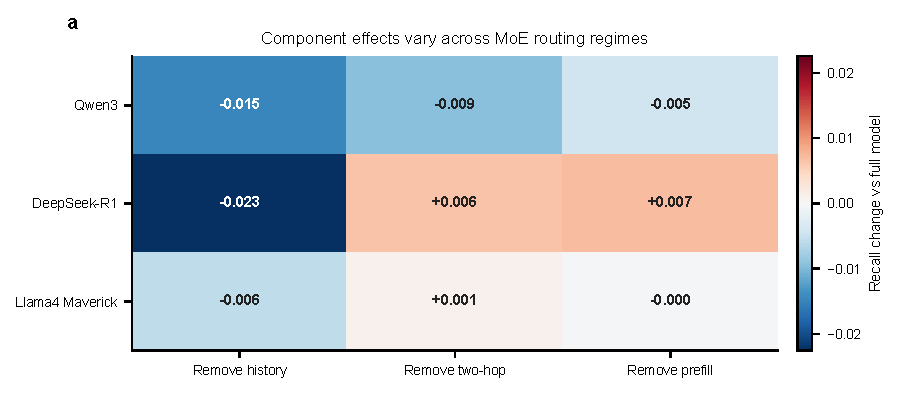
\includegraphics[width=\linewidth]{figures_final/Fig4_ComponentAblation}
\end{minipage}
\caption{Development-scale budget and component analyses. Left:
coverage--waste trade-offs as the fixed candidate width increases; dotted
lines denote native \(K\). Right: native-budget Recall change after removing
individual route-evidence components.}
\label{fig:budget}
\label{fig:ablation}
\end{figure*}

\subsection{Component Utility Depends on the Routing Regime}

Ablation on the development-scale evaluation revealed heterogeneous branch utility
(Fig.~\ref{fig:ablation}). Removing route history reduced native-budget Recall
by 0.0148 on Qwen3, 0.0226 on DeepSeek-R1, and 0.0056 on Llama 4 Maverick.
It was the only tested removal that degraded every model. Two-hop and
request-prefill evidence benefited Qwen3 but did not generalize uniformly.
Removing either branch improved DeepSeek-R1 by 0.0064 and 0.0069,
respectively. The evidence supports context-conditioned weighting of
complementary signals, but not universal benefit from every branch.

\subsection{Marginal Calibration Supports Score-Mass Selection}

The fitted temperatures were 0.82 for Qwen3, 0.32 for DeepSeek-R1, and 1.05
for Llama 4 Maverick. On the development-scale test split, scaling reduced ECE from
0.2894 to 0.2801 for Qwen3 and from 0.3827 to 0.2763 for DeepSeek-R1
(Fig.~\ref{fig:calibration-budget}a). Llama 4 Maverick instead showed a small
increase from 0.1236 to 0.1250. Temperature scaling therefore improved
marginal calibration most strongly for DeepSeek-R1, but did not improve it
uniformly. Because temperature preserves score ordering, these changes did not
constitute an additional ranking gain.

Validation selected cumulative score masses of 0.70, 0.95, and 0.50 for Qwen3,
DeepSeek-R1, and Llama 4 Maverick, respectively
(Fig.~\ref{fig:calibration-budget}b). The resulting mean candidate widths were
11.75, 17.25, and 6.56, with validation Recall of 0.6120, 0.3786, and 0.6293.
DeepSeek-R1 required the widest candidate set but retained the lowest Recall.
These values are operating thresholds over normalized ranking weights, not
nominal coverage probabilities. The operating points show that a single
score-mass threshold cannot represent all three routing regimes.

\begin{figure}[!t]
\centering
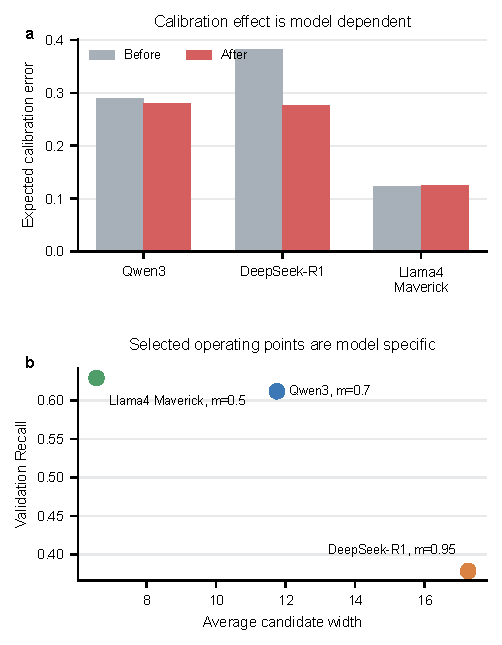
\includegraphics[width=0.96\columnwidth]{figures_final/Fig5_CalibrationSelection}
\caption{Development-scale marginal calibration and adaptive-budget selection. (a)
Marginal expected calibration error before and after per-model temperature scaling;
lower is better. (b) Validation-selected operating points. Labels denote
cumulative score mass, and coordinates report mean candidate width and Recall.}
\label{fig:calibration-budget}
\end{figure}

\subsection{Selective Scheduling Changes Idealized Cache-Replay Outcomes}

Idealized cache-event replay separated expert coverage from the transfer count
of acting on predictions
(Fig.~\ref{fig:cache-pareto}). On Qwen3, the adaptive-cache policy reached hit
rates of 0.5345, 0.7197, and 0.8771 at \(1\times\), \(2\times\), and
\(4\times\) capacity. It required 1.00, 0.62, and 0.31 million total
transfers, respectively. Relative to unfiltered adaptive-mass prefetching,
cache-aware admission reduced transfers by 53--62\%. At \(4\times\), it
retained a hit rate of 0.8771 rather than 0.8775 while avoiding approximately
0.10 million transfers. At \(1\times\), fixed native-budget prefetching
produced the higher hit rate, exposing a tight-capacity rejection cost.

DeepSeek-R1 formed the clearest failure case. Fixed native-budget prefetching
achieved the highest hit rate at every tested capacity. Cache-aware admission
reduced transfers relative to adaptive mass, but did not recover the lost hit
rate. For Llama 4 Maverick, adaptive cache achieved the highest hit rate at
\(2\times\) and \(4\times\) while using fewer transfers than adaptive mass.
Demand-only LRU nevertheless required the fewest transfers. Selective
admission therefore improved the quality of speculative movement without
dominating every policy on both cache hits and transfer count.

The transfer reduction was most useful when admission preserved or improved
residency. At \(4\times\) capacity, DeepSeek-R1 adaptive cache reduced total
transfers from 1.66 million to 0.79 million relative to adaptive mass, while
its hit rate increased slightly from 0.4282 to 0.4309. Llama 4 Maverick showed
a stronger joint improvement at the same capacity: transfers decreased from
187,345 to 74,188, while hit rate increased from 0.5521 to 0.5569. By contrast,
the tight-cache Qwen3 result traded hit rate for fewer and more selective
transfers. Cache-aware admission therefore changed the operating point rather
than producing a uniform improvement in either metric alone.

Prefetch Precision helps explain why fewer transfers did not translate
monotonically into a higher hit rate. At \(1\times\) capacity, Qwen3
adaptive-cache admission raised prefetch Precision from 0.3808 under fixed
native-budget prefetching to 0.5397, although its hit rate remained lower. At
\(4\times\), the fixed policy instead achieved the higher Precision (0.6120
versus 0.4978), while adaptive admission retained nearly the same hit rate as
unfiltered adaptive mass with substantially fewer transfers. DeepSeek-R1
showed a different pattern: at \(4\times\), adaptive-cache and fixed-budget
Precision were similar (0.2962 and 0.2895), yet the fixed policy still obtained
the higher hit rate. For Llama 4 Maverick, adaptive-cache Precision decreased
from 0.2493 at \(1\times\) to 0.1245 at \(4\times\), even though the larger
caches improved demand hit rate. Prefetch Precision and residency benefit must
therefore be reported separately.

The replay results expose three operating regimes. Qwen3 is
admission-sensitive under a tight cache: filtering removes many transfers but
can reject experts that would soon be reused. DeepSeek-R1 is primarily
forecast-limited, so scheduling cannot compensate for its weaker expert
ranking. Llama 4 Maverick is budget-sensitive because native Top-1 routing
makes each unnecessary candidate proportionally expensive, yet additional
capacity allows selective admission to improve hit rate. These regimes explain
why one cache policy does not dominate across models and capacities. They also
motivate selecting the admission rule jointly with model family and cache
capacity rather than treating cache awareness as a model-independent
post-processing step.

\begin{figure}[!t]
\centering
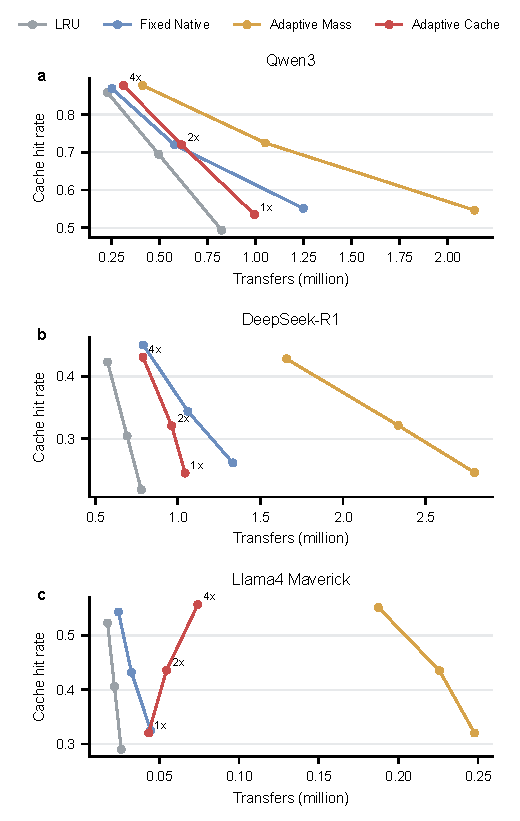
\includegraphics[width=0.96\columnwidth]{figures_final/Fig6_CachePareto}
\caption{Development-scale idealized cache-event replay for (a) Qwen3, (b)
DeepSeek-R1, and (c) Llama 4 Maverick. Curves contain capacities of
\(1\times\), \(2\times\), and \(4\times\). Upper-left positions combine
higher hit rate with fewer expert transfers.}
\label{fig:cache-pareto}
\end{figure}

\FloatBarrier

\section{Discussion}

RouteCast separates two requirements that are often conflated in expert
prefetching: forecasting the next route and deciding whether a forecast merits
movement. Its native-budget gains show that route history contains predictive
structure beyond heatmaps, GRUs, and TCNs. The budget sweeps, however, show
that greater coverage can require many false transfers. Forecast quality and
prefetch utility are therefore related but non-equivalent objectives.

The branch ablations refine this conclusion. Recent route history was useful
for every model, whereas two-hop and request-prefill evidence had
model-dependent effects. Conditional fusion is valuable because it can
suppress unreliable evidence, not because every branch helps universally.
Likewise, one shared checkpoint retained nearly the macro Recall of three
independent predictors, but shared training did not improve every model.
Group-DRO contributed no measurable numerical advantage in the single-seed
ablation. These outcomes indicate shared route structure alongside
architecture-specific regularities.

Calibration and scheduling exposed a second form of heterogeneity.
DeepSeek-R1 required the widest candidate set and remained the least
predictable, while every additional Llama 4 Maverick candidate imposed a large
Precision cost under native Top-1 routing. Temperature scaling adjusted score
concentration but could not recover information absent from route history.
Operating thresholds must therefore be selected and audited per routing
regime.

Cache-aware admission is complementary to router co-design, proactive loading,
and sparsity-aware caching \cite{pregated,moeinfinity,promoe}. It supplies a
runtime with ranked candidates but does not replace the native router. The
idealized Pareto frontiers show that filtering can reduce transfer
amplification, although no policy dominated every model and cache capacity.
Weak forecasts and tight caches both limit the value of speculative movement.

The route-only constraint provides portability but imposes a performance
ceiling. Discrete traces support training across heterogeneous MoE families,
yet omit hidden states and router logits that may explain abrupt route changes.
A hidden-state-aware method could achieve higher Recall, but would require a
different deployment interface and comparison setting.

Three limitations bound the conclusions. First, idealized cache-event replay
omits transfer deadlines, kernel scheduling, bandwidth contention,
transfer--compute overlap, throughput, and energy. It cannot establish
end-to-end acceleration. Second, component, calibration, adaptive-budget, and
cache analyses use the 100-request-per-model development-scale evaluation;
the primary 1,000-request-per-model evaluation covers forecasting, baselines,
and cross-model training. Third, the matched learned comparators include GRU
and TCN models but not an equivalent-input transformer. End-to-end deployment,
large-scale scheduling, and a matched attention baseline remain open tests.

\section{Conclusion}

RouteCast provides a route-only pipeline from next-token expert forecasting to
selective prefetch action. Its context-conditioned gate combines statistical
and temporal evidence without accessing hidden states or modifying the native
router. Model-specific marginal calibration and validation-selected score mass
convert the predicted ranking into an adaptive candidate set, while low-weight
rejection and cache-aware admission
control which candidates trigger speculative movement.

Across request-disjoint traces from Qwen3, DeepSeek-R1, and Llama 4 Maverick,
RouteCast exceeded the matched TCN baseline by 2.81, 4.55, and 5.79 percentage
points under the respective native routing budgets. Paired request-level
bootstrap intervals excluded zero for all three comparisons. One shared
checkpoint was within 0.0007 macro Recall of three per-model predictors, while
Group-DRO did not provide a numerical gain. Development-scale
analyses further showed that increasing coverage can reduce Precision and
amplify transfers. Cache-aware admission moved selected operating points
toward fewer transfers, although the preferred policy depended on model and
cache capacity.

These findings support RouteCast as a reproducible algorithmic interface
between route forecasting, adaptive candidate selection, and expert-cache
management. They do not establish that RouteCast accelerates a deployed MoE
system. Confirming latency, throughput, energy, and overlap benefits requires
integration with a serving runtime and measurement on representative
offloading hardware.

\appendix
\section{Development-Scale Seed Stability}

The primary forecasting tables use training seed 2026 and quantify uncertainty
by resampling complete test requests. We additionally assessed whether the
RouteCast--TCN difference depended on one optimization seed. RouteCast and the
matched TCN baseline were trained with seeds 2024, 2025, and 2026 on the
100-request-per-model development-scale evaluation. Split membership remained fixed
because request assignment is determined by the request-path hash rather than
the training seed.

\begin{figure}[H]
\centering
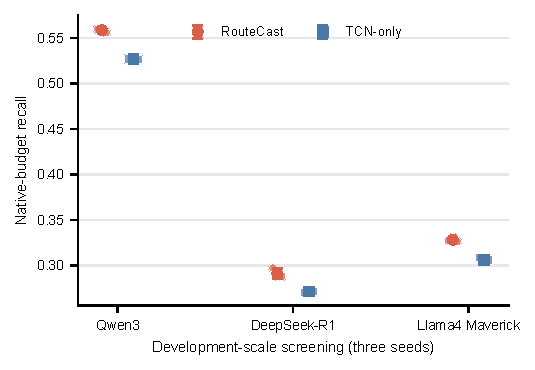
\includegraphics[width=0.82\columnwidth]{figures_final/FigS1_SeedStability}
\caption{Development-scale optimization stability over seeds 2024--2026.
Small points denote individual runs; large markers and error bars denote mean
\(\pm\) sample standard deviation. RouteCast exceeds TCN-only for all nine
model--seed combinations.}
\label{fig:tcn-seeds}
\end{figure}

RouteCast exceeded TCN-only for all nine model--seed combinations
(Fig.~\ref{fig:tcn-seeds}). Its mean native-budget Recall advantage was
\(0.0317\pm0.0017\) on Qwen3, \(0.0196\pm0.0062\) on DeepSeek-R1, and
\(0.0219\pm0.0041\) on Llama 4 Maverick, where uncertainty denotes the sample
standard deviation across three seeds. This screening indicates that the
observed advantage was not confined to one initialization. Because it uses
only three seeds and the smaller development-scale evaluation, it complements rather
than replaces the request-level bootstrap on the primary evaluation.

\begin{thebibliography}{00}
\bibitem{shazeer2017} N. Shazeer, A. Mirhoseini, K. Maziarz, A. Davis,
Q. V. Le, G. E. Hinton, and J. Dean, ``Outrageously large neural networks:
The sparsely-gated mixture-of-experts layer,'' in \emph{Proc. Int. Conf.
Learn. Represent. (ICLR)}, 2017.

\bibitem{gshard} D. Lepikhin et al., ``GShard: Scaling giant models with
conditional computation and automatic sharding,'' in \emph{Proc. Int. Conf.
Learn. Represent. (ICLR)}, 2021.

\bibitem{switch} W. Fedus, B. Zoph, and N. Shazeer, ``Switch Transformers:
Scaling to trillion parameter models with simple and efficient sparsity,''
\emph{J. Mach. Learn. Res.}, vol. 23, no. 120, pp. 1--39, 2022.

\bibitem{pregated} R. Hwang et al., ``Pre-gated MoE: An algorithm-system
co-design for fast and scalable mixture-of-expert inference,'' in
\emph{Proc. 51st ACM/IEEE Int. Symp. Comput. Archit. (ISCA)}, 2024,
pp. 1018--1031, doi: 10.1109/ISCA59077.2024.00078.

\bibitem{moeinfinity} L. Xue, Y. Fu, Z. Lu, L. Mai, and M. Marina,
``MoE-Infinity: Efficient MoE inference on personal machines with
sparsity-aware expert cache,'' arXiv:2401.14361, 2024.

\bibitem{promoe} X. Song, Z. Zhong, R. Chen, and H. Chen, ``ProMoE: Fast
MoE-based LLM serving using proactive caching,'' arXiv:2410.22134, 2024.

\bibitem{patterns} Z. Yu et al., ``Patterns behind chaos: Forecasting data
movement for efficient large-scale MoE LLM inference,'' arXiv:2510.05497,
2025.

\bibitem{deepspeedmoe} S. Rajbhandari et al., ``DeepSpeed-MoE: Advancing
mixture-of-experts inference and training to power next-generation AI scale,''
in \emph{Proc. 39th Int. Conf. Mach. Learn. (ICML)}, 2022,
pp. 18332--18346.

\bibitem{tutel} C. Hwang et al., ``Tutel: Adaptive mixture-of-experts at
scale,'' in \emph{Proc. Mach. Learn. Syst.}, vol. 5, 2023.

\bibitem{fiddler} K. Kamahori, T. Tang, Y. Gu, K. Zhu, and B. Kasikci,
``Fiddler: CPU--GPU orchestration for fast inference of mixture-of-experts
models,'' in \emph{Proc. Int. Conf. Learn. Represent. (ICLR)}, 2025.

\bibitem{stmoe} Y. Zhao, R. Bunescu, A. Louri, A. Karanth, and K. Wang, ``A
spatio-temporal expert prefetching framework for efficient MoE-based LLM
inference,'' arXiv:2606.15453, 2026.

\bibitem{specmd} D. Hoang, A. Jaiswal, M. Samragh, and M. Cho, ``SpecMD: A
comprehensive study on speculative expert prefetching,'' arXiv:2602.03921,
2026.

\bibitem{specprefetch} J. Kong et al., ``SpecPrefetch: Parameter-efficient
expert prefetching for sparse MoE foundation models,'' arXiv:2607.24787,
2026.

\bibitem{cho2014} K. Cho, B. van Merri\"enboer, C. Gulcehre, D. Bahdanau,
F. Bougares, H. Schwenk, and Y. Bengio, ``Learning phrase representations
using RNN encoder--decoder for statistical machine translation,'' in
\emph{Proc. Conf. Empirical Methods Natural Lang. Process. (EMNLP)}, 2014,
pp. 1724--1734, doi: 10.3115/v1/D14-1179.

\bibitem{sagawa2020} S. Sagawa, P. W. Koh, T. B. Hashimoto, and P. Liang,
``Distributionally robust neural networks for group shifts: On the importance
of regularization for worst-case generalization,'' in \emph{Proc. Int. Conf.
Learn. Represent. (ICLR)}, 2020.

\bibitem{loshchilov2019} I. Loshchilov and F. Hutter, ``Decoupled weight
decay regularization,'' in \emph{Proc. Int. Conf. Learn. Represent. (ICLR)},
2019.

\bibitem{guo2017} C. Guo, G. Pleiss, Y. Sun, and K. Q. Weinberger, ``On
calibration of modern neural networks,'' in \emph{Proc. 34th Int. Conf. Mach.
Learn. (ICML)}, 2017, pp. 1321--1330.

\bibitem{bai2018} S. Bai, J. Z. Kolter, and V. Koltun, ``An empirical
evaluation of generic convolutional and recurrent networks for sequence
modeling,'' arXiv:1803.01271, 2018.

\bibitem{jarvelin2002} K. J\"arvelin and J. Kek\"al\"ainen, ``Cumulated
gain-based evaluation of IR techniques,'' \emph{ACM Trans. Inf. Syst.},
vol. 20, no. 4, pp. 422--446, 2002,
doi: 10.1145/582415.582418.

\bibitem{efron1993} B. Efron and R. J. Tibshirani, \emph{An Introduction to
the Bootstrap}. New York, NY, USA: Chapman \& Hall, 1993.
\end{thebibliography}

\end{document}
